Infrastruktura je sačinjena od servera, čvorova, usmjerivača i sl.
Također, infrastrukturu čini operacijski sustav, vatrozid, i ostali softver\cite{ibm-infrastructure}.
Po tom pitanju danas se ništa značajno nije promijenilo, samo su fizičke komponente skrivene u "oblaku" (eng. \textit{cloud}).
Rad zahtjeva vrlo jednostavnu infrastrukturu pa je oblak prikladno rješenje jer ne zahtjeva vlastoručnu konfiguraciju i održavanje fizičkih komponenti.

\begin{figure}[h!]
    \centering
    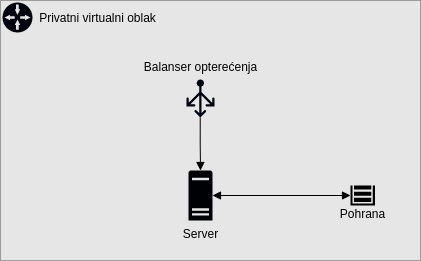
\includegraphics[scale=0.7]{images/infrastructure}
    \caption{Fizičke komponente infrastrukture}
    \label{fig:physical-infrastructure}
\end{figure}

Na slici~\ref{fig:physical-infrastructure} nalaze se sve komponente kreirane kod pružatelja usluge oblaka (DigitalOcean).
Privatni virtualni oblak ima mnoštvo značajki, ali u ovom slučaju se koristi samo za logičko grupiranje komponenti.
Balanser opterećenja (eng. \textit{load balancer}) služi kao \textit{proxy} do glavnog servera i moguće je povezati domenu na njega.
Server ima vlastitu sekundarnu pohranu na kojoj se nalazi operacijski sustav i potrebni alati ali i vanjsku pohranu na kojoj se nalaze aplikacijski podaci.

Vanjska pohrana i balanser opterećenja izgledaju, na prvi pogled, nepotrebni.
U scenariju kad se glavni server nepovratno sruši vrlo je lako kreirati novi i nastaviti s normalnim radom.
Krajnji korisnik osjeti kratki prekid usluge, a ne potpuni gubitak usluge i podataka.
U slučaju samo jednog servera (bez vanjske pohrane i balansera opterećenja) podaci i IP adresa se trajno gube što predstavlja veliku
neugodnost krajnjem korisniku.

\subsection{Infrastruktura aplikacije}

Moderne aplikacije zahtijevaju različite servise i alate kako bi funkcionirale u potpunosti.
Baza podataka, red čekanja, posrednik poruka i web server samo su neki od servisa.
Potrebni su alati za ažuriranje, objavljivanje i nadzor aplikacija i servisa.

Danas je najpopularniji način objavljivanja aplikacija pomoću kontejnera.
Kontejner je rezultat procesa pakiranja aplikacijskog koda sa svim potrebnim bibliotekama i alatima kako bi ga se moglo
lako i pouzdano prenositi između okruženja, npr.\ lokalno (na računalu programera), testno (\textit{staging}) i
stvarno (\textit{production})~\cite{docker-containers}.

Sam kontejner nema nikakvu funkciju dok se ne pokrene.
Kontejneri nisu izvršne datoteke (\textit{.exe}) da ih operacijski sustav može pokrenuti bez dodatnih alata.
Čak i kad bi operacijski sustav to mogao, kontejner je moguće zaustaviti, ponovno pokrenuti, može završiti u stanju
greške (eng. \textit{error state}) te je potrebna "logika" kad i kako treba poduzeti određene akcije.
Operacijski sustav se bavi puno nižim stvarima pa problem upravljanja kontejnerom izlazi iz domene operacijskog sustava.

Aplikacije su uglavnom sačinjene od više modula i servisa pa je potrebno i više kontejnera.
Ručno upravljanje s istima je vremenski i resursno zahtjevan proces, ali postoje alati koji olakšavaju upravljanje kontejnerima.
To su alati koji pomažu pri orkestriranju kontejnera (eng. \textit{container orchestration}) i jedan od njih je i \textit{Kubernetes}.
Kubernetes je sustav koji pomaže pri automatiziranju procesa objave i ažuriranja, skaliranja i sveukupnog
upravljanja aplikacijama i servisima~\cite{kubernetes}.

Razmjer praktičnog rada ne zahtjeva mnoštvo značajki koje Kubernetes nudi, samo osnovnu značajku:
grupira kontejnere koji čine aplikaciju u logičke jedinice~\cite{kubernetes}.
To omogućava lakše razumijevanje komponenti sustava kao i vizualizaciju istih.

\pagebreak

\begin{figure}[h!]
    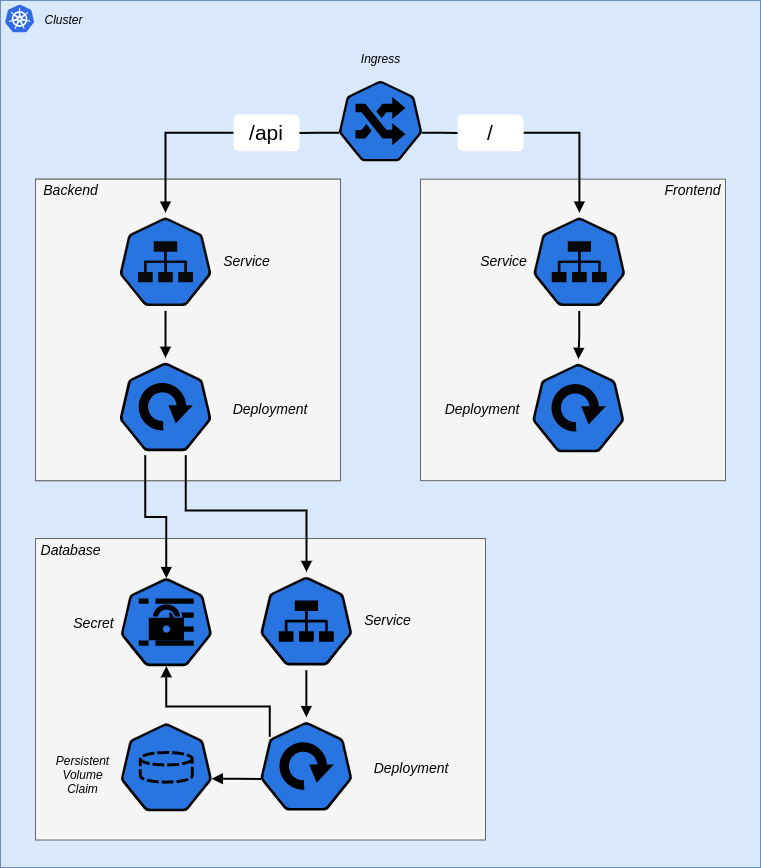
\includegraphics[width=\textwidth]{images/app-infrastructure}
    \caption{Servisi i komponente sustava}
    \label{fig:application-infrastructure}
\end{figure}

Na slici~\ref{fig:application-infrastructure} je prikazan \textit{cluster} sa svim servisima i komponentama.
Početna točka je \textit{ingress} koji funkcionira kao \textit{proxy}.
Ovisno o putanji koju korisnik zahtjeva, zahtjev se prosljeđuje na \textit{backend} (pozadinska aplikacija) ili \textit{frontend} (grafičko sučelje).

Grafičko sučelje se sastoji od dvije komponente: \textit{Service} i \textit{Deployment}.
\textit{Deployment} zna kako pokrenuti kontejner, kad je kontejner spreman za obradu zahtjeva i koliko replika ima.
Kako svaki kontejner ima svoju IP adresu ostali servisi bi morali znati točnu IP adresu kontejnera
kako bi ga mogli koristiti.
\textit{Service} predstavlja apstrakciju nad kontejnerima i ponaša se kao balanser opterećenja (u slučaju više replika)
ili \textit{proxy} (u slučaju jedne replike).

Pozadinska aplikacija je slična grafičkom sučelju osim što ovisi o bazi podataka.
Ovisi o \textit{Service} komponenti baze podataka kao i pristupnim podacima koji se nalaze u komponenti \textit{Secret}.
Kako bi pozadinska aplikacija komunicirala s bazom podataka potrebno je nekoliko podataka:
\begin{itemize}
    \item Adresa
    \item Korisničko ime
    \item Lozinka
    \item Naziv baze podataka
\end{itemize}

Kako je već rečeno da je \textit{Service} apstrakcija nad kontejnerima tako je sam naziv servisa ujedno i \textbf{adresa}.
\textbf{Korisničko ime}, \textbf{lozinka} i \textbf{naziv baze podataka} se nalaze u \textit{Secret} komponenti.
Ona predstavlja jedini izvor točnosti (eng. \textit{single source of truth}) pa ukoliko dođe do promjena
u podacima pozadinska aplikacija i baza podataka mogu pravilno reagirati kako bi nesmetano funkcionirali.

Baza podataka, naspram pozadinske aplikacije, ima jednu komponentu više: \textit{Persistent Volume Claim}.
Svaki kontejner ima sustav datoteka odvojen od domaćinovog sustava datoteka (eng. \textit{host file system}).
U slučaju zaustavljanja kontejnera (namjerno ili uslijed greške) svi podaci bi bili trajno izgubljeni.
Kako bi se to izbjeglo potrebno je dozvoliti kontejneru pisanje u domaćinov sustav datoteka.
Komponenta \textit{Persistent Volume Claim} apstrahira ovu funkcionalnost pa sam kontejner uopće ne zna da se podaci zapravo
zapisuju na domaćinov sustav datoteka.
To omogućava djelomično fizičko odvajanje domaćinovog sustava datoteka.
Direktoriji koji su potrebni bazi podataka su odvojeni na vanjsku pohranu (slika~\ref{fig:physical-infrastructure}) dok su
podaci i datoteke o kojima ovisi operacijski sustav pohranjeni na internu pohranu servera.
U slučaju nepovratnog pada servera (npr.~fizičko oštećenje) zamjenom servera sustav nastavlja raditi bez gubitka podataka.
